\subsection*{RESEARCH PROJECT}
% - Describe how the research is significant and how it addresses an important problem
% - Describe how the Proposal meets the objectives of the Discovery Projects scheme
% - Describe how the anticipated outcomes will advance the knowledge base of the discipline and
%   how the Proposal aims and concepts are novel and innovative
% - Outline the conceptual framework, design and methods and demonstrate that these are
%   adequately developed, well integrated and appropriate to the aims of the Proposal. Include
%   research plans and proposed timelines
% - Detail what new methodologies or technologies will be developed in the course of the research
%   and how they will advance knowledge
% - Outline the feasibility of the project, in terms of design, budget and proposed timeline
% - If the rationale for some of the Proposal rests upon manuscripts that are still in the process of
%   being published, or on results of work that may not be available to assessors, include a
%   summary of the relevant work
% - Describe the expected outcomes and likely impact of the proposed research
% - Describe how the Proposal might result in national or international economic, commercial,
%   environmental, social and/or cultural benefits
% - If the research has been nominated as focussing upon a topic or outcome that falls within one
%   of the Science and Research Priorities, describe the potential for the project to contribute to the associated Priority Goals.

The January 2011 Brisbane River floods in south-east Queensland cost
32 lives and caused 2.5~billion dollars worth of
damage~\parencite{vandenhonert2011}. In the days leading up to
these events, a key issue facing authorities was incorporating their
\textbf{uncertainty} about the preceding fortnight's rainfall into the
modelling. In their report on the causes, impacts and implications of
the floods, \cite{vandenhonert2011} concluded:
\blockquote{whilst the dam operators were acting in accordance with
  the operations manual for the dam, their modelling did not take
  account of forecast rainfall in determining the predicted dam water
  level, and this resulted in a sub-optimal water release strategy.
  Employing tools for decision making under uncertainty would have
  resulted in a different water release strategy.} At the other end of
the environmental spectrum, bushfire model predictions are similarly
\textquote[\cite{alexanderLimitations2013} p375]{fraught with
  uncertainty}. As Australia's climate changes and extreme weather
events become more common, there is a significant need for better ways
to gather timely insights from modelling in the presence of
uncertainty and to communicate those insights to decision makers and
emergency services.

Computational modelling and simulation is an invaluable support tool
for disaster response, allowing emergency services personnel to
explore what might happen in the immediate future under various
scenarios. But these model simulations can be fraught with
uncertainty: some of their \emph{input parameters} may be well known
(possibly from reliable sensor data), others may be known only
approximately, and others still may only be guessed at. Even with
perfect input data, the models themselves entail assumptions and
numerical approximations which bound the reliability of their
predictions.

\subsubsection*{The Modelling Problem}

More formally, suppose that we have a mathematical model
$M_{\mathbf{p}}$ parameterised by the vector
$\mathbf{p}\in\mathcal{P}$. For example, $M_{\mathbf{p}}$ may be a
parameterised partial differential equation %(PPDE)
in a storm surge model. For each $\mathbf{p}$ we suppose the model is
well-defined and there exists a unique function
\begin{equation}
  \label{eq:1}
  U_{\mathbf{p}}(\mathbf{x})\, \quad \mathbf{x}\in\Omega
\end{equation}
which is a solution to the model problem, that is $M_{\mathbf{p}}(U_{\mathbf{p}})=0$.
Here the \emph{domain space} $\Omega$ represents variables such as 
time and space, 
and $U_{\mathbf{p}}$ represents scalar or vector fields of interest, 
such as storm surge water level and/or velocity.    

Sometimes the goal of the modeller is to better understand the
relationship between $\mathbf{p}$ and some lower-dimensional quantity
of interest $Q(U_{\mathbf{p}})$, such as the relationship between a
particular rainfall scenario and the maximum storm surge levels at
particular geographical locations. In order to achieve such
understanding, repeated executions of the model (or approximations of the model solution) are often required
with an expert analysis of the outputs of each stage and selection of
the next parameter set based on an assessment of those outputs. Such
repeated model executions can also be used to estimate the
\emph{uncertainty} in any given set of predictions of
$Q(U_{\mathbf{p}})$. Through the process of trying different model
parameterisations, the scientist is able to build up an understanding
of the \emph{general} relationship between $\mathbf{p}$ and
$Q(U_{\mathbf{p}})$, including the areas of the parameter space
$\mathcal{P}$ which have the greatest influence on the result and
which types of uncertainty have the greatest impact on the certainty
of the results.

\paragraph*{A specific storm-surge example:}
Consider the problem of predicting the maximum 
storm surge water level along a coast threatened by a cyclone. 
A mathematical model of storm surge is provided 
by the shallow water wave equation,  which encodes the conservation of water and Newton's second Law (Force = mass $\times$ acceleration) 
\begin{align*}
\frac{\partial h}{\partial t} +
\frac{\partial }{\partial x} \left(uh\right) + \frac{\partial }{\partial y} \left(vh\right) &= R, \\
\frac{\partial uh}{\partial t} +
\frac{\partial }{\partial x} \left(u^2h  \frac12 gh^2 \right) 
+ \frac{\partial }{\partial y} \left(vuh\right) &= - gh \frac{\partial b}{\partial x} 
+ \frac{h}{\rho} \frac{\partial P}{\partial  x} + S_{fx} + S_{wx} ,\\
\frac{\partial vh}{\partial t} +
\frac{\partial }{\partial x} \left(uvh  \right) 
+ \frac{\partial }{\partial y} \left(v^2h + \frac12 g h^2 \right) &=  - gh \frac{\partial b}{\partial y} 
+ \frac{h}{\rho} \frac{\partial P}{\partial  y} + S_{fy} + S_{wy},
\end{align*}
where $h(x,y,t)$ is the depth of water, $u(x,y,t)$ and $v(x,y,t)$ are the $x$ and $y$ horizontal components of water velocity, $g$ is the gravitational constant (9.81), $\rho$ is the density of water, $b(x,y)$ is the bathymetry (elevation of the ocean bed), $R$ is the rate of rainfall, $P$ is the atmospheric pressure (which generates a surge due to spatial differences in atmospheric pressure associated with a large cyclone), $S_{fx}$ and $S_{fy}$ are the $x$ and $y$ components of the frictional force generated by the flow of the surge over the ocean bed (flow over sand is different than flow through mangroves) , and $S_{wx}$ and $S_{wy}$ are the $x$ and $y$ components of the surface stress force (generated by the wind). As is evident, there are many opportunities for uncertainty in the data defining this model. 
As demonstrated in our papers~\parencite{anugamanual,nielsen2005hydrodynamic}  these
equations and their implementation in the AnuGA package provide a reliable
model of general flows associated with inundation due to riverine flooding, storm-surge 
and tsunamis.

The parameter space $\mathcal{P}$ needs to represent the variation in the input data $R$, $b$, $P$, $S_f$, $S_w$, as well as design parameters describing actions such as raising or lowering flood barriers and releasing or diverting flow from upstream rivers, or flood basins, or indeed constructing emergency levees. 
The domain $\Omega$ represents the variables $x$, $y$ over a geographical region and $t$ over a time interval, such as a  coastal region threatened by a cyclone over particular time interval. The model solution 
$$
U_{\mathbf{p}} (\mathbf{x})  = \begin{bmatrix} h(x,y,t) \\ u(x,y,t) \\ v(x,y,t) \end{bmatrix}
$$
represents the water depth and velocity fields obtained by solving the model problem for a particular value of the parameter $\mathbf{p}$ (or perhaps a high fidelity numerical approximation of this problem). 

A quantity of interest $Q(U_{\mathbf{p}})$ could be the maximum storm surge height at a particular location $(x_0, y_0)$
$$ 
Q(U_{\mathbf{p}})  = \max_{t_0 \leq t \leq t_1} \left( h(x_0,y_0,t) + b(x_0,y_0) \right).
$$
The aim of  uncertainty quantification is to obtain useful relationships between the variations in pressure, wind and rainfall  and $Q(U_{\mathbf{p}})$, including the which components of the inputs  which have the greatest influence on the result. 




%or to find the parameter choice $\mathbf{p}$
%which optimises $Q$. %over all $\mathbf{x}$.
%This high-level description of the ``model selection/optimisation''
% workflow 
%(shown
%graphically in Figure~\ref{fig:general-fb-loop})
 %lies at the heart of
%a great deal of modern science.
%\begin{figure}
 % \centering
  %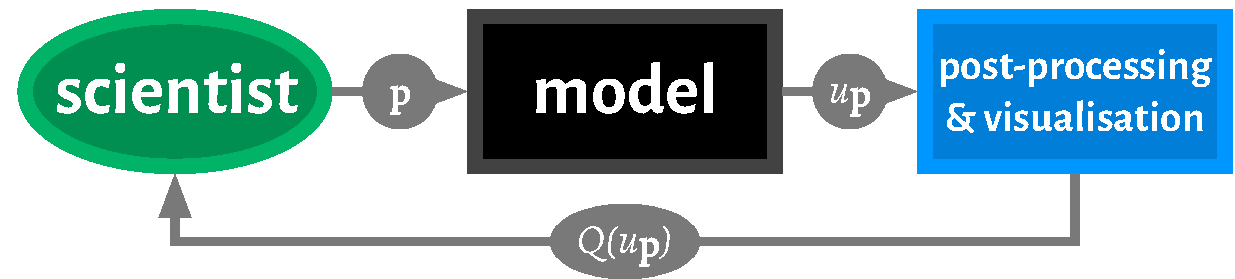
\includegraphics[width=.6\textwidth]{figures/general-fb-loop.pdf}
  %\caption{The human-in-the-loop modelling workflow. A scientist
    %selects an initial parameter $\mathbf{p_0}$ for their model,
    %examines the model output $Q(u_{\mathbf{p}})$, and either accepts
    %the output of the model or re-runs the model with a different
    %choice of the parameter $\mathbf{p_1}$.}
  %\label{fig:general-fb-loop}
%\end{figure}
%There are many ways of finding an optimal $\mathbf{p}$, from 
%trial-and-error experimentation to expert judgement through to fully-automated algorithmic
%optimization procedures. Often there are ways to optimise $\mathbf{p}$
%algorithmically, although these methods often introduce new parameters (the
%arguments of the function being optimised) which must be selected by the
%scientist. 
%As a result, this feedback loop will often require many
%iterations, with a scientist-in-the-loop, evaluating the results
%of the model (possibly through visualising the model output) and
%choosing a parameter update $\Delta\mathbf{p}$ at each step.
% (see
%Figure~\ref{fig:unrolled-fb-loop}). 
%Each step through this loop
%provides feedback to the scientist about the response of the system to
%a particular value of $\mathbf{p}$ --  for example, the maximum storm
%surge level under a particular rainfall scenario. 

%\begin{figure}
% \centering
%  
\includegraphics[width=\textwidth]{figures/unrolled-fb-loop.pdf}
%  \caption{If the modelling \& post-processing/visualisation steps can
%    be performed sufficiently quickly, then the scientist can explore
%    the $\mathbf{p} \rightarrow Q(u_{\mathbf{p}})$ relationship
%    \emph{interactively}, with the all the associated benefits for
%    exploratory analysis.}
%  \label{fig:unrolled-fb-loop}
%\end{figure}

From a workflow perspective, the productivity of the
modeller/scientist is proportional to the rate at which they can
explore the $\mathbf{p} \rightarrow Q(U_{\mathbf{p}})$ relationship.
Any latency improvements in this feedback loop will translate into
productivity gains~\parencite{liuEffects2014}. If the model
parameters $\mathbf{p}$ and inputs $\mathbf{x}$ are known precisely
and the quantity $Q(U_{\mathbf{p}})$ is cheap to calculate and easy to
interpret, then the task is simple: provide the scientist with an
interface for manipulating $\mathbf{p}$ and set them loose. However,
for real-world models (such as those used in flood/storm
surge/bushfire modelling) this is often not the case. There are
\textbf{three primary challenges}:
\begin{enumerate}
\item \emph{The model may not provide a way to express uncertainty in
    the inputs}. Many models do not provide methods for including
  uncertainty information in their inputs, as was the case in the 2011
  Brisbane River flood example.
\item \emph{The quantity $Q(U_{\mathbf{p}})$ may not be cheap to
    calculate}. Many
  sophisticated models require non-trivial computing resources 
  to evaluate. These compute resources may be
  difficult to secure, with submitted jobs having to wait in a queue, 
  and may
  take a long time to compute even when the resources are available.
  This is especially problematic in a disaster-response scenario,
  where an approximately correct answer provided in a short time is
  significantly more useful than a perfect answer provided after it is
  too late to act on.
\item \emph{The quantity $Q(U_{\mathbf{p}})$ together with estimates
    of its uncertainty may not be easy to interpret}. Oftentimes this
  is a visualisation problem--- the mapping
  $\mathbf{p} \rightarrow Q(U_{\mathbf{p}})$ may be high-dimensional,
  and presenting that to a decision-maker, particularly when combining
  it with its uncertainty estimates, may not be straightforward.
\end{enumerate}
%\begin{figure}
 % \centering
  %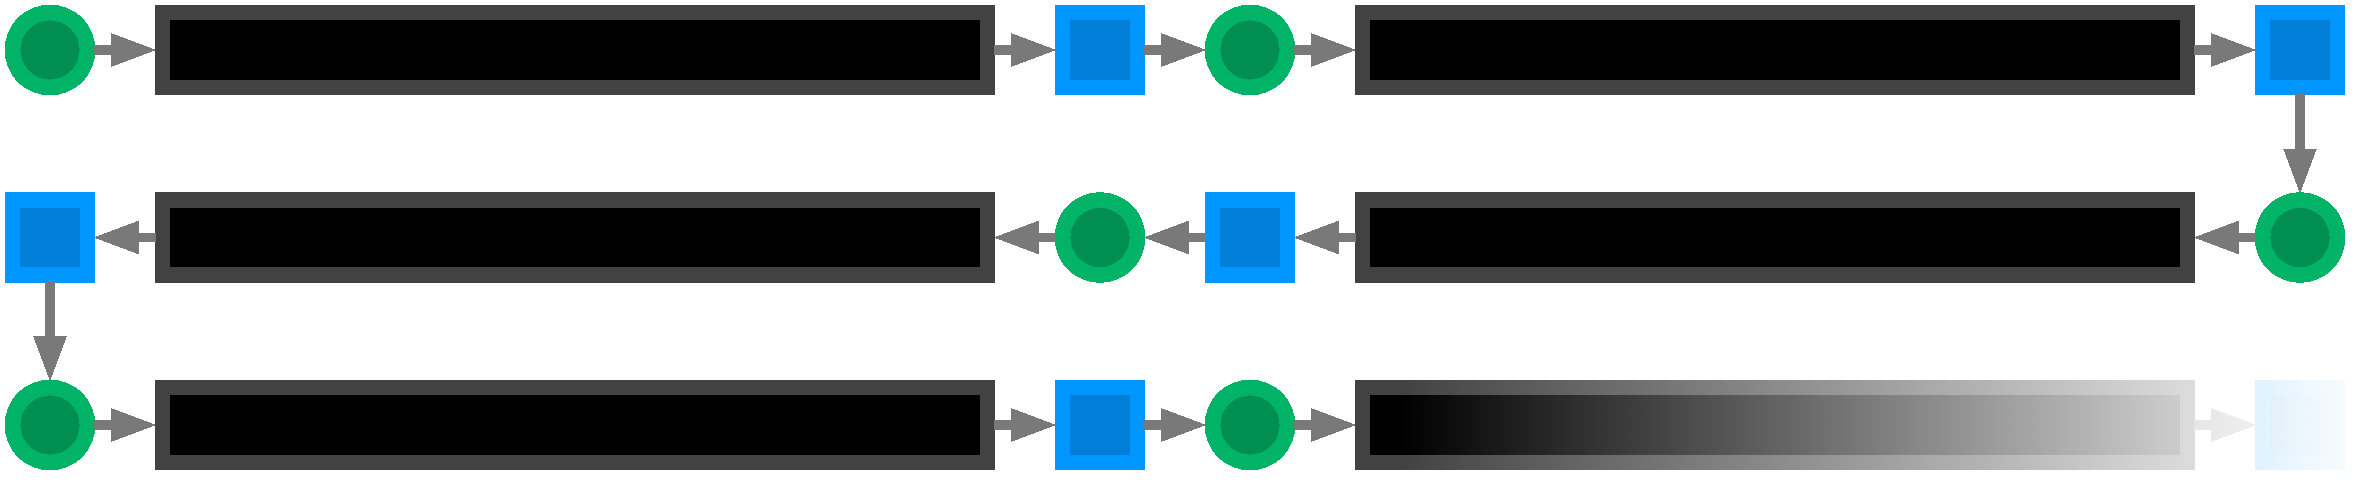
\includegraphics[width=\textwidth]{figures/long-fb-loop.pdf}
  %\caption{If the model is computationally expensive to run, then the
   % workflow is dominated by waiting for the model to finish. This
    %results in lower productivity---not only due to the time spent
    %waiting for the model, but also because of the temporal separation
  %between the selection of a new parameter $\mathbf{p}$, and seeing
 % its impact on the results of the model.}
 % \label{fig:long-fb-loop.pdf}
%\end{figure}



\subsubsection*{Live Coding for Uncertainty
  Quantification}

This project will
make use of the \emph{Extempore} live-coding software
environment.%\footnote{\url{http://extempore.moso.com.au}}
 Extempore has already
been used for the live modification and real-time visualisation of
particle-in-cell plasma-physics simulation codes with
negligible performance overhead compared to batch-mode execution in
C~\parencite{swiftLive2016}. 



Such a live deployment of a traditional, batch-oriented HPC simulation allows a user to 
modify the
domain size and shape, the initial and boundary conditions, and various
other parameters of a simulation while that simulation is running. It is of use
for optimising software for later, stand-alone,
deployment as well as for harnessing and steering simulation codes
after deployment.

%The Extempore software environment is a key tool for this project as
%it allows us to fine tune our suite of simulation software for the
%specific requirements of the task domain.

The ability to stop, modify, or restart computations `in flight' has
the potential to significantly improve the efficiency of an
uncertainty analysis. There exist many algorithms, for example
adaptive Markov chain Monte Carlo methods~\parencite{GilksEtal1994}, 
which attempt to choose the best samples based on the sampling
history. For complex problems however, a domain expert
may often have
a better idea about the region of the parameter domain where function
evaluations should be concentrated. Through live programming within a
tight feedback loop a domain expert can incrementally guide the
current sampling strategy being used for uncertainty 
quantification, and in turn be guided by 
real time information derived from the reduced order model 
(such as surpluses
provided by sparse grid approximation to 
identify important parameter dimensions and regions of interest), 
to improve the end result. The resulting strategies are expected to be
more aggressive in nature as they are better targeted to the specific
problem at hand. The result of this should be more efficient quantification of
uncertainty.

In this project, using live coding to accelerate the feedback loop between the vector of input parameters,
$\mathbf{p}$,  and quantities of interest  will give a scientist the ability to interactively
\emph{explore} the connection (and the associated uncertainty) between
the different dimensions of $\mathbf{p}$ and the overall response of
the system. Such a prototyping and optimising of these models ({\bf Aim 2 of our project}) will help us rapidly scope and deliver 
robust models. The ``liveness'' that this approach brings will also be deployed 
into the uncertainty quantification models. For example, reduced-basis methods for uncertainty 
quantification typically employ a number of ``offline'' simulations that are used together with an ``online'' simulation of 
a system of interest to provide uncertainty estimates for that online simulation; we will apply novel live-coding
approaches to such methods where the offline as well as the online simulations are all harnessed and live. The 
potential advantage of such an approach is that the offline simulations can be restarted, modified, reduced and 
explored at the same time that the online simulation is running. Such a research agenda in live coding is one that 
includes human-computer interaction (HCI) as well as software engineering. HCI research questions include the realistic time-scales of 
human-in-the-loop interaction with running simulation software, both for software development and for decision making in real time.
HCI research methodologies will include ethnographic studies and protocol analysis of ``staged'' interaction scenarios including
human actors. We will be looking to identify states of interaction 
of expert users with our live-coding systems as well as transitions between them -- much as we have already done so in the 
context of computer music~\parencite{swift2014coding}.






%This will be used to {\bf rapidly prototype software} with a view to 
%dentifying the necessary interactive controls needed to modify and interact with 
%the final, relased and running, software in real-time. 
%By understanding the human-factors and systems-level time
%constraints on the delivery of useful information in disaster-response
%settings, we will also be able to specify timing requirements on our model
%simulations as in the next section. 
%By developing software that is time-constrained and
%time-aware, we will be able to provide decision makers with
%information when it is needed and with an estimate on the uncertainty
%of that information.
%Ultimately, the scientist needs an \textbf{interactive interface} for
%gleaning insights from their models in the presence of these
%challenges.
%\newpage

%\begin{figure}
 % \centering
  %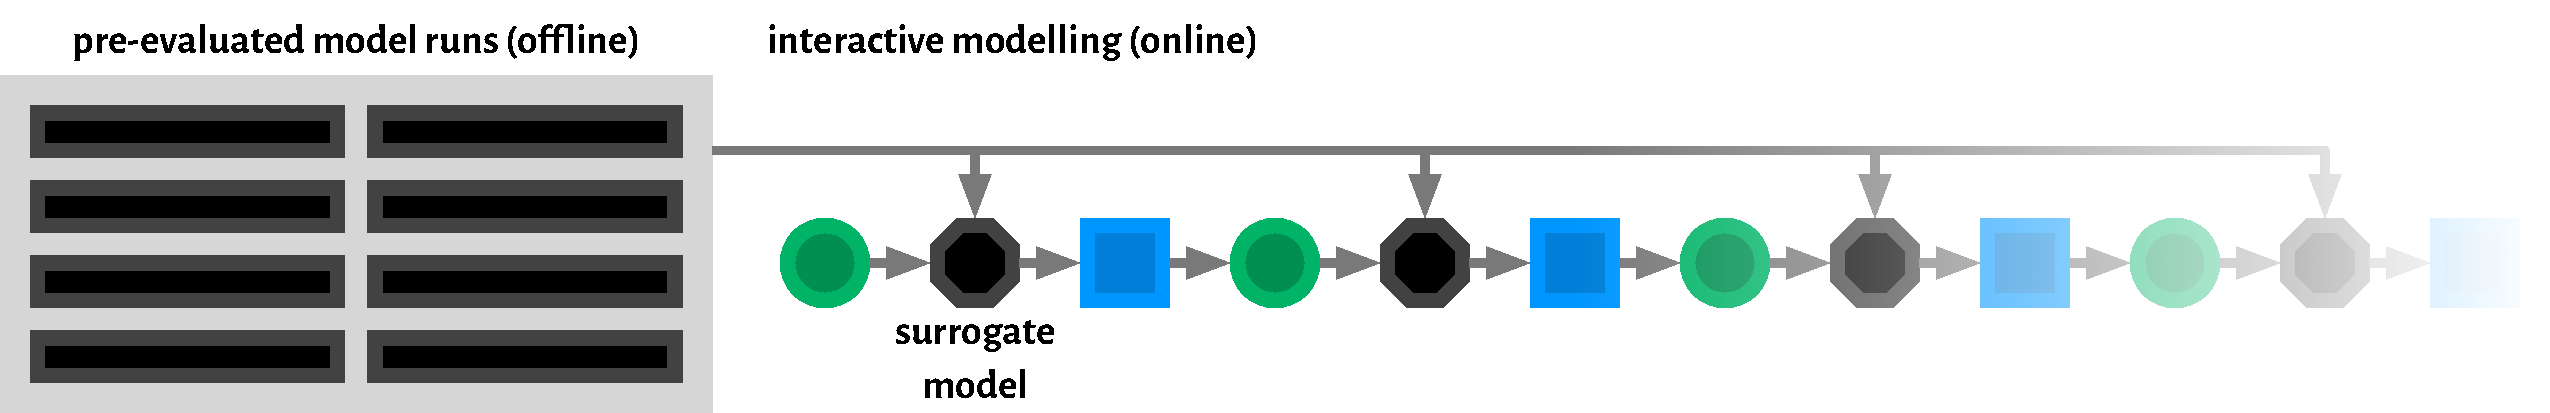
\includegraphics[width=\textwidth]{figures/sg-surrogate-model-fb-loop.pdf}
  %\caption{Using the sparse grids and reduced basis models, the computationally
   % expensive model calculations can be done ahead-of-time and used to
    %construct a surrogate model which can be used to re-claim the
    %interactive workflow of Figure~\ref{fig:unrolled-fb-loop}}.
  %\label{fig:sg-surrogate-model-fb-loop}
%\end{figure}

%Impact: new algorithms, software, high performance computer systems
%and visualisation techniques for time-bound environmental simulation
%with uncertainty. New software tools for the simulation of flood
%surges and tsunami. New methodologies for rapid and agile software
%development and usability using live programming. New knowledge of
%human-in-the-loop requirements for support systems in the context of
%environmental disaster management. New algorithms, software, high
%performance computer systems and visualisation techniques for
%time-bound environmental simulation with uncertainty. New software
%tools for the simulation of flood surges and tsunami. New
%methodologies for rapid and agile software development and usability
%using live programming. New knowledge of human-in-the-loop
%requirements for support systems in the context of environmental
%disaster management.




\subsubsection*{Sparse-Grids and Uncertainty Quantification}

The mathematical component of this project will be based on new
developments combining sparse
grids~\parencite{BungartzGriebel2004}, reduced basis
methods~\parencite{LiebermanEtal2010,Peherstorfer2013,ChenSchwab2015,PeherstorferWillcox2015}
and uncertainty quantification. One of the main difficulties in the
study of current scientific models is the high dimensional spaces
involved, often both in the parameter and domain spaces, $\mathcal{P}$
and $\Omega$ respectively. This is a significant barrier for the
timely evaluation of models due to the `curse of dimensionality' in
which the cost scales exponentially with dimension. By using sparse
grids and reduced basis models we will be able to compute
\emph{surrogates of the full problem} which have significantly fewer
unknowns and are thus cheaper to compute whilst maintaining a high
order of accuracy. For example, a general approach would be to find a
lower dimensional manifold of the parameter space
$\mathcal{Q}\subset\mathcal{P}$ over which the model is most sensitive
using a proper orthogonal decomposition. A sparse grid surrogate of
the model over $\mathcal{Q}$ can also be computed in an offline phase,
so that in an online phase model solutions can be efficiently
estimated using the surrogate model. For many problems sparse grids
can also be used over $\Omega$ when computing solutions to the full
model to speed up the construction of a reduced basis. We will compute
sparse grid solutions via the `combination
technique'~\parencite{Griebel1990}. Figure~\ref{fig:sparse_grids}
depicts the combination technique, the equivalent sparse grid and the
corresponding full grid.

\begin{figure}
  \centering
  % Brendan: combination grid, sparse grid, fullgrid figure

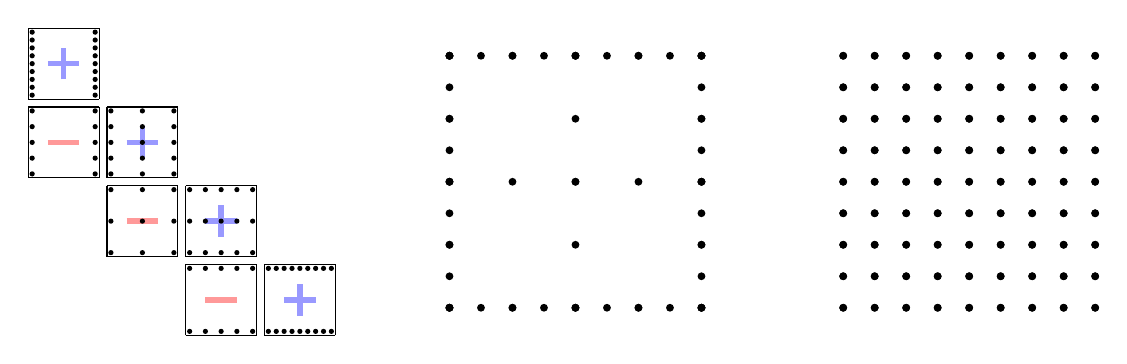
\begin{tikzpicture}%[scale=0.8]
%\scriptsize
%%% Draw squares around component grids
\foreach \i in {1,...,4}
{
	\pgfmathtruncatemacro{\x}{(\i - 1)};
	\draw[] (0.05+1.0*\x, 3.05-1.0*\x) -- (0.05+1.0*\x+0.9, 3.05-1.0*\x) {};
	\draw[] (0.05+1.0*\x, 3.05-1.0*\x) -- (0.05+1.0*\x, 3.05-1.0*\x+0.9) {};
	\draw[] (0.05+1.0*\x+0.9, 3.05-1.0*\x) -- (0.05+1.0*\x+0.9, 3.05-1.0*\x+0.9) {};
	\draw[] (0.05+1.0*\x, 3.05-1.0*\x+0.9) -- (0.05+1.0*\x+0.9, 3.05-1.0*\x+0.9) {};
	%%% optional plotting of coefficients
	\draw[blue!40,line width=0.7mm] (0.5+1.0*\x-0.2, 3.0+0.5-1.0*\x) -- (0.5+1.0*\x+0.2, 3.0+0.5-1.0*\x);
	\draw[blue!40,line width=0.7mm] (0.5+1.0*\x, 3.0+0.5-1.0*\x-0.2) -- (0.5+1.0*\x, 3.0+0.5-1.0*\x+0.2);
}
\foreach \i in {1,...,3}
{
	\pgfmathtruncatemacro{\x}{(\i - 1)};
	\draw[] (0.05+1.0*\x, 2.05-1.0*\x) -- (0.05+1.0*\x+0.9, 2.05-1.0*\x) {};
	\draw[] (0.05+1.0*\x, 2.05-1.0*\x) -- (0.05+1.0*\x, 2.05-1.0*\x+0.9) {};
	\draw[] (0.05+1.0*\x+0.9, 2.05-1.0*\x) -- (0.05+1.0*\x+0.9, 2.05-1.0*\x+0.9) {};
	\draw[] (0.05+1.0*\x, 2.05-1.0*\x+0.9) -- (0.05+1.0*\x+0.9, 2.05-1.0*\x+0.9) {};
	%%% optional plotting of coefficients
	\draw[red!40,line width=0.7mm] (0.5+1.0*\x-0.2, 2.0+0.5-1.0*\x) -- (0.5+1.0*\x+0.2, 2.0+0.5-1.0*\x);
}
%%% Combination grids
\foreach \i in {1,...,18} %2*9
{
	\pgfmathtruncatemacro{\y}{(\i - 1) / 2};
	\pgfmathtruncatemacro{\x}{\i - 1 - 2 * \y};
	\node[fill,circle,scale=0.2] at (0.1+0.8*\x,3.1+0.1*\y) {};
	\node[fill,circle,scale=0.2] at (3.1+0.1*\y,0.1+0.8*\x) {};
}
\foreach \i in {1,...,15} %3*5
{
	\pgfmathtruncatemacro{\y}{(\i-1)/3};
	\pgfmathtruncatemacro{\x}{\i-1-3*\y};
	\node[fill,circle,scale=0.2] at (1.1+0.4*\x,2.1+0.2*\y) {};
	\node[fill,circle,scale=0.2] at (2.1+0.2*\y,1.1+0.4*\x) {};
}
\foreach \i in {1,...,10} %2*5
{
	\pgfmathtruncatemacro{\y}{(\i-1)/2};
	\pgfmathtruncatemacro{\x}{\i-1-2*\y};
	\node[fill,circle,scale=0.2] at (0.1+0.8*\x,2.1+0.2*\y) {};
	\node[fill,circle,scale=0.2] at (2.1+0.2*\y,0.1+0.8*\x) {};
}
\foreach \i in {1,...,9} %3*3
{
	\pgfmathtruncatemacro{\y}{(\i - 1) / 3};
	\pgfmathtruncatemacro{\x}{\i - 1 - 3 * \y};
	\node[fill,circle,scale=0.2] at (1.1+0.4*\x,1.1+0.4*\y) {};
}
%%% Sparse grid
\foreach \i in {1,...,18} %2*9
{
	\pgfmathtruncatemacro{\y}{(\i - 1) / 2};
	\pgfmathtruncatemacro{\x}{\i - 1 - 2 * \y};
	\node[fill,circle,scale=0.3] at (5.4+3.2*\x,0.4+0.4*\y) {};
	\node[fill,circle,scale=0.3] at (5.4+0.4*\y,0.4+3.2*\x) {};
}
\foreach \i in {1,...,15} %3*5
{
	\pgfmathtruncatemacro{\y}{(\i-1)/3};
	\pgfmathtruncatemacro{\x}{\i-1-3*\y};
	\node[fill,circle,scale=0.3] at (5.4+1.6*\x,0.4+0.8*\y) {};
	\node[fill,circle,scale=0.3] at (5.4+0.8*\y,0.4+1.6*\x) {};
}
%%% Full grid
\foreach \i in {1,...,81} %9*9
{
	\pgfmathtruncatemacro{\y}{(\i - 1) / 9};
	\pgfmathtruncatemacro{\x}{\i - 1 - 9 * \y};
	\node[fill,circle,scale=0.3] at (10.4+0.4*\x,0.4+0.4*\y) {};
	\node[fill,circle,scale=0.3] at (10.4+0.4*\y,0.4+0.4*\x) {};
}
\end{tikzpicture}  
  \caption{Combination grids on the left (with coefficients, marked with
    a blue plus for $+1$ and red minus for $-1$), sparse grid in the
    middle, full grid on the right. Note the marked reduction in the number of 
    grid points for the sparse grid relative to the full grid. 
   This is even more pronounced in higher dimensions.}
  \label{fig:sparse_grids}
\end{figure}

Propagating uncertainty in scientific models which are high
dimensional and/or expensive to compute is a significant challenge.
For models which are not stochastic in nature, and thus have no means
of directly quantifying uncertainty, one must typically estimate
statistical moments via Monte Carlo methods or quadrature rules. For
high dimensional problems it has been shown that sparse grids can
estimate these moments faster and more accurately than traditional
Monte Carlo methods when the probability density functions are
sufficiently
smooth~\parencite{JakemanRoberts2013,FranzelinDiehlPfluger2014}.
Despite the advantages of reduced basis methods, the manifold
$\mathcal{Q}$ is still sufficiently high dimensional that the
quantification of uncertainty remains a challenge due to the sheer
number of function evaluations required. This is particularly true
when the quantification of uncertainty in a model is a component of an
optimisation algorithm. As such it is important to continue to
develop efficient numerical methods for uncertainty quantification
for high dimensional problems. Replacing the full model with a reduced
basis model also adds additional error and uncertainties. One needs to
have some idea what the model outcomes may be for parameters not lying
on the lower dimensional manifold $\mathcal{Q}$. An important part of
developing reduced models is `verifying' the model, by bounding their
error of the surrogate for example. By using ensemble methods,
multifidelity models~\parencite{NgWillcox2014} and gradient enhanced
approximation~\parencite{deBaarHarding2015,Jakeman2015} we hope to
improve the verification and propagation of uncertainties in models.
Incorporating ideas from `Kriging' (Gaussian process regression), a
feature of which is having confidence intervals over an interpolant,
together with sparse-grid interpolation, we will be able to express
uncertainties explicitly in the surrogate model.



\subsubsection*{Live Coding of Scientific Simulation}

\iffalse
Live coding is a term which has been used to denote systems which
support the direct intervention of the programmer in a program's
run-time state. It can be thought of as an extreme version of the
agile programming methodology~\parencite{fowlerAgile2001}, where
code changes are hot-swapped into running programs, allowing for
extremely fast exploration and iteration of new ideas and system
updates. As the ambition of live-coding has grown, support systems and
languages have evolved to, for example, create, modify and interact
with music and hardware devices in real time. Such an approach has
been termed `\emph{with-time}
programming'~\parencite{sorensen2010programming}. 
\fi

This project will
make use of the \emph{Extempore} software
environment\footnote{\url{http://extempore.moso.com.au}} which has
been used for live modification and real-time visualisation of
particle-in-cell (PIC) plasma physics simulation codes, with
negligible performance overhead compared to batch-mode execution in
C~\parencite{swiftLive2016}. This allows the scientist to modify the
domain size/shape, the initial and boundary conditions, and various
other parameters while the simulation is running, with live visual
feedback.

The Extempore software environment is a key tool for this project as
it allows us to fine tune our suite of simulation software for the
specific requirements of the task domain.




\subsubsection*{From Disaster-Response Human-Factors Optimisation to Software Development}

% GOMS model for co-operative scenarios where someone wants
% information, and someone is trying to present it to them

% it's about chunking complex tasks c.f. beginning-middle-end

% the goal: quantitative requirements on the time bounds, which has
% implications for the design of the systems

Similar to ~\parencite{ramchurn2016human} we will employ game
scenarios to understand and optimise collaboration for disaster
response~\parencite{ramchurn2016human}. However, our focus will be on
decision-maker/modeller communication rather than human/agent
communication and our game scenarios will take place while software
and systems parameters, particularly the human-computer interface,
visualisations and system configuration, are being tuned in real time
by a live coder. In a novel approach, the protocols obtained from this
live coding will then be analysed to determine macro ``chunking''
states, of human action and transitions between those states. We have
recently used similar approaches to understand the real-time actions
of single live-coders in computer music
performance~\parencite{swift2014coding} and the macro-gesture states
of group computer musicians using
iPads~\parencite{martin2015tracking}. In both of these studies,
transition matrices derived from interaction protocols were able to
yield insights into the artistic process. In the case of the present
project, data from the interaction protocols of the live-coder will be
feed back into redesign of the software interface and the controls
needed for the computational platform.

By way of one simple example, we imagine that, perhaps, the live coder
finds that a particular measure of uncertainty, \emph{measure-A}, is
routinely requested by a decision maker after another particular
measure, \emph{measure-B}. The live coder could tune up the software
in real time so that these two measures could be presented together.
The interaction protocols in this instance might reveal insights into
the \emph{context} where these two measures were requested one after
the other and the software might be redesigned to recognise that
context and to make the two measures accessible in that context. For
another simple example, the live-coding protocol might show that data
processing needed to be occasionally shifted from one part of a cloud
resource to a local cluster. Examination of these instances could
impact on the computer systems settings needed to properly deploy
these simulations. Our approach to protocol analysis will go well
beyond simple examples like these and will use matrix theory to derive
insights into the nature of state transitions across entire protocols
and across test participants.



\subsubsection*{Interactive Design Optimisation}

The methodology we will develop for this project will also have
significant benefits for engineering design. We will explore this in
the context of design optimisation problems from aerospace and
aeronautics. Design optimisation poses a significant challenge due to
the large number of input parameters, for example in describing the
geometry of an airfoil, and there are a number of ways in which
uncertainty comes into the modelling. For example, the manufacturing
process is not exact, and the full range of attack angles, velocities,
stresses and weather conditions the airfoil will be exposed to during
flight can only be guessed at. In this project we will build on our
previous work in applying sparse grid methods in airfoil
design~\parencite{SU2,deBaarHarding2015}, using an interactive
feedback loop to improve the efficiency of the design process within
our live coding and uncertainty quantification framework.




\subsubsection*{High-Performance Computing Systems Support}

A reliance on high performance computing for the evaluation of
scientific models provides additional challenges to the technical side
of the project. Specifically, our algorithms must be highly scalable
and robust to errors and faults in the computer system layer. There
have been many recent developments in both highly-scalable algorithms
and the sparse grid combination technique \cite{sgctalg15,pdsec15extsgctalg} 
which will be of use for
this and, additionally, it has been recently shown that such
computations can be made
robust~\parencite{HardingHLS2015,AliEtal2015,Ali11022016}. By leveraging and
continuing to develop these algorithms we can ensure that the
offline components of our software system that require high performance
computing resources will be both scalable and robust.

In this project we will leverage on-demand compute resources, such as
the Amazon AWS cloud~\parencite{amazonAws} and the National Compute
Infrastructure NCI Cloud~\parencite{nciCloud}. Using these cloud
services will further improve the project's ability to deliver timely
results in high-pressure and time-critical decision making scenarios.

Once again, we emphasise that our approach to live coding of test
software is a novel aspect of our methodology. The \emph{Extempore}
tool that we have developed has been shown to be able to harness and
steer scientific simulation in real time. In this part of the project,
we will apply this tool to the real-time steering of the computer
systems layer itself.

This will involve developing code libraries to assist the developer in
the live performance evaluation and tuning of these complex and highly
parallel simulations. For example, groups of processes will be
allocated to different parts of the simulation. If some parts are
delayed relative to others, processes can be `stolen' from the faster
group to improve load balance \cite{parSGCT16}. Communication
bottlenecks can be identified and alternate communication algorithms
can be employed to rectify this.  Different computational kernels can
be selected depending on the current memory system and floating point
performance.  It should be noted that this fine-tuning is not only
application-dependent, but within an application, it depends on the
workload selected, and even within that, may depend on the current
phase of the simulation. Only Live Programming by \emph{Extempore} has
the flexibility and agility to facilitate such a degree of performance
tuning.


\subsubsection*{Interactive Visualisation of Environmental Forecasts with Uncertainty}

Similar to the impact of visually presented geodata on decision
making~\parencite{kinkeldey2015evaluating}, the particular
visualisations of uncertainty in our environmental models will need to
be systematically evaluated with human participants. Here we will
adopt traditional human-factors trials with non-expert participants
together with qualitative feedback from emergency services experts. We
will solicit qualitative feedback from expert participants from
emergency authorities in our local area including ACT Emergency
Service, Geosciences Australia, the Australian Maritime and Safety
Authority and the Australian Federal Police. Perspectives offered by
this participant pool will be important in extrapolating our study
results to real world disaster-management.



